% Created by tikzDevice version 0.6.2-92-0ad2792 on 2013-03-23 23:04:02
% !TEX encoding = UTF-8 Unicode
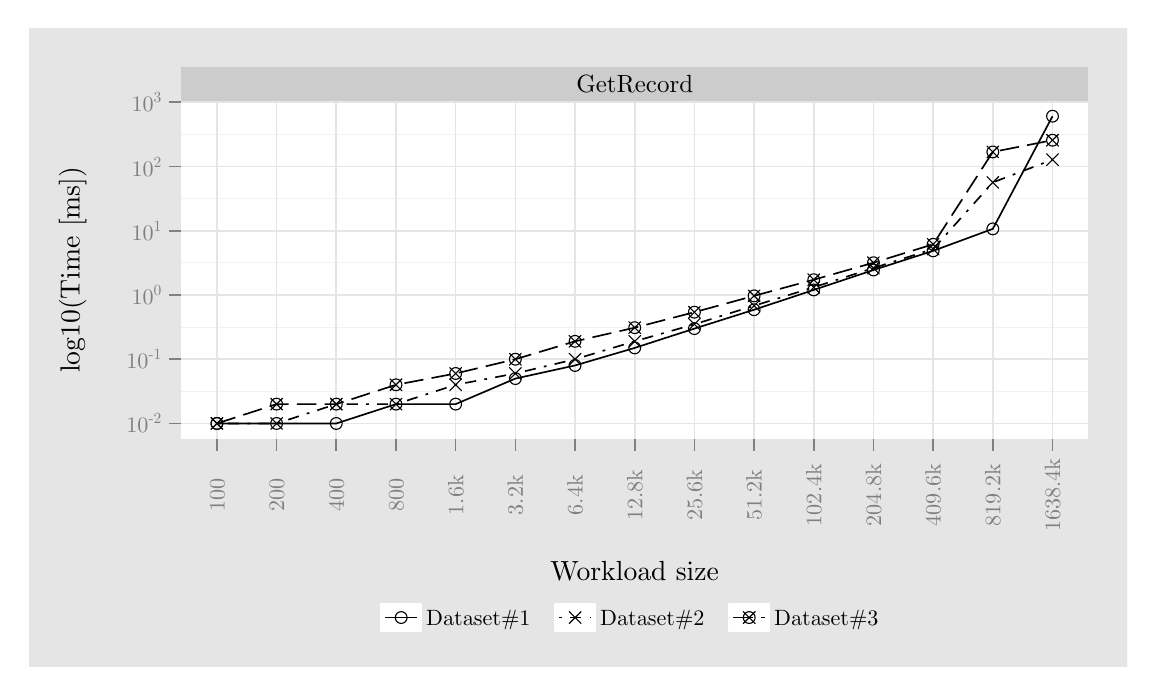
\begin{tikzpicture}[x=1pt,y=1pt]
\definecolor[named]{fillColor}{rgb}{1.00,1.00,1.00}
\path[use as bounding box,fill=fillColor,fill opacity=0.00] (0,0) rectangle (397.48,231.26);
\begin{scope}
\path[clip] (  0.00,  0.00) rectangle (397.48,231.26);
\definecolor[named]{drawColor}{rgb}{1.00,1.00,1.00}
\definecolor[named]{fillColor}{rgb}{0.90,0.90,0.90}

\path[draw=drawColor,line width= 0.6pt,line join=round,line cap=round,fill=fillColor] (  0.00,  0.00) rectangle (397.48,231.26);
\end{scope}
\begin{scope}
\path[clip] ( 55.45, 82.69) rectangle (383.26,204.82);
\definecolor[named]{fillColor}{rgb}{1.00,1.00,1.00}

\path[fill=fillColor] ( 55.45, 82.69) rectangle (383.26,204.82);
\definecolor[named]{drawColor}{rgb}{0.95,0.95,0.95}

\path[draw=drawColor,line width= 0.3pt,line join=round] ( 55.45, 99.85) --
	(383.26, 99.85);

\path[draw=drawColor,line width= 0.3pt,line join=round] ( 55.45,123.05) --
	(383.26,123.05);

\path[draw=drawColor,line width= 0.3pt,line join=round] ( 55.45,146.26) --
	(383.26,146.26);

\path[draw=drawColor,line width= 0.3pt,line join=round] ( 55.45,169.47) --
	(383.26,169.47);

\path[draw=drawColor,line width= 0.3pt,line join=round] ( 55.45,192.68) --
	(383.26,192.68);
\definecolor[named]{drawColor}{rgb}{0.90,0.90,0.90}

\path[draw=drawColor,line width= 0.6pt,line join=round] ( 55.45, 88.24) --
	(383.26, 88.24);

\path[draw=drawColor,line width= 0.6pt,line join=round] ( 55.45,111.45) --
	(383.26,111.45);

\path[draw=drawColor,line width= 0.6pt,line join=round] ( 55.45,134.66) --
	(383.26,134.66);

\path[draw=drawColor,line width= 0.6pt,line join=round] ( 55.45,157.86) --
	(383.26,157.86);

\path[draw=drawColor,line width= 0.6pt,line join=round] ( 55.45,181.07) --
	(383.26,181.07);

\path[draw=drawColor,line width= 0.6pt,line join=round] ( 55.45,204.28) --
	(383.26,204.28);

\path[draw=drawColor,line width= 0.6pt,line join=round] ( 68.39, 82.69) --
	( 68.39,204.82);

\path[draw=drawColor,line width= 0.6pt,line join=round] ( 89.95, 82.69) --
	( 89.95,204.82);

\path[draw=drawColor,line width= 0.6pt,line join=round] (111.52, 82.69) --
	(111.52,204.82);

\path[draw=drawColor,line width= 0.6pt,line join=round] (133.09, 82.69) --
	(133.09,204.82);

\path[draw=drawColor,line width= 0.6pt,line join=round] (154.65, 82.69) --
	(154.65,204.82);

\path[draw=drawColor,line width= 0.6pt,line join=round] (176.22, 82.69) --
	(176.22,204.82);

\path[draw=drawColor,line width= 0.6pt,line join=round] (197.79, 82.69) --
	(197.79,204.82);

\path[draw=drawColor,line width= 0.6pt,line join=round] (219.35, 82.69) --
	(219.35,204.82);

\path[draw=drawColor,line width= 0.6pt,line join=round] (240.92, 82.69) --
	(240.92,204.82);

\path[draw=drawColor,line width= 0.6pt,line join=round] (262.49, 82.69) --
	(262.49,204.82);

\path[draw=drawColor,line width= 0.6pt,line join=round] (284.05, 82.69) --
	(284.05,204.82);

\path[draw=drawColor,line width= 0.6pt,line join=round] (305.62, 82.69) --
	(305.62,204.82);

\path[draw=drawColor,line width= 0.6pt,line join=round] (327.19, 82.69) --
	(327.19,204.82);

\path[draw=drawColor,line width= 0.6pt,line join=round] (348.75, 82.69) --
	(348.75,204.82);

\path[draw=drawColor,line width= 0.6pt,line join=round] (370.32, 82.69) --
	(370.32,204.82);
\definecolor[named]{drawColor}{rgb}{0.00,0.00,0.00}

\path[draw=drawColor,line width= 0.6pt,line join=round] ( 68.39, 88.24) --
	( 89.95, 88.24) --
	(111.52, 88.24) --
	(133.09, 95.23) --
	(154.65, 95.23) --
	(176.22,104.46) --
	(197.79,109.20) --
	(219.35,115.54) --
	(240.92,122.52) --
	(262.49,129.34) --
	(284.05,136.49) --
	(305.62,143.69) --
	(327.19,150.61) --
	(348.75,158.56) --
	(370.32,199.27);

\path[draw=drawColor,line width= 0.6pt,dash pattern=on 1pt off 3pt on 4pt off 3pt ,line join=round] ( 68.39, 88.24) --
	( 89.95, 88.24) --
	(111.52, 95.23) --
	(133.09, 95.23) --
	(154.65,102.21) --
	(176.22,106.30) --
	(197.79,111.45) --
	(219.35,117.92) --
	(240.92,124.08) --
	(262.49,130.77) --
	(284.05,137.45) --
	(305.62,144.40) --
	(327.19,151.27) --
	(348.75,175.34) --
	(370.32,183.56);

\path[draw=drawColor,line width= 0.6pt,dash pattern=on 7pt off 3pt ,line join=round] ( 68.39, 88.24) --
	( 89.95, 95.23) --
	(111.52, 95.23) --
	(133.09,102.21) --
	(154.65,106.30) --
	(176.22,111.45) --
	(197.79,117.92) --
	(219.35,122.85) --
	(240.92,128.45) --
	(262.49,134.35) --
	(284.05,140.18) --
	(305.62,146.32) --
	(327.19,152.98) --
	(348.75,186.35) --
	(370.32,190.59);

\path[draw=drawColor,line width= 0.4pt,line join=round,line cap=round] ( 68.39, 88.24) circle (  2.13);

\path[draw=drawColor,line width= 0.4pt,line join=round,line cap=round] ( 89.95, 88.24) circle (  2.13);

\path[draw=drawColor,line width= 0.4pt,line join=round,line cap=round] (111.52, 88.24) circle (  2.13);

\path[draw=drawColor,line width= 0.4pt,line join=round,line cap=round] (133.09, 95.23) circle (  2.13);

\path[draw=drawColor,line width= 0.4pt,line join=round,line cap=round] (154.65, 95.23) circle (  2.13);

\path[draw=drawColor,line width= 0.4pt,line join=round,line cap=round] (176.22,104.46) circle (  2.13);

\path[draw=drawColor,line width= 0.4pt,line join=round,line cap=round] (197.79,109.20) circle (  2.13);

\path[draw=drawColor,line width= 0.4pt,line join=round,line cap=round] (219.35,115.54) circle (  2.13);

\path[draw=drawColor,line width= 0.4pt,line join=round,line cap=round] (240.92,122.52) circle (  2.13);

\path[draw=drawColor,line width= 0.4pt,line join=round,line cap=round] (262.49,129.34) circle (  2.13);

\path[draw=drawColor,line width= 0.4pt,line join=round,line cap=round] (284.05,136.49) circle (  2.13);

\path[draw=drawColor,line width= 0.4pt,line join=round,line cap=round] (305.62,143.69) circle (  2.13);

\path[draw=drawColor,line width= 0.4pt,line join=round,line cap=round] (327.19,150.61) circle (  2.13);

\path[draw=drawColor,line width= 0.4pt,line join=round,line cap=round] (348.75,158.56) circle (  2.13);

\path[draw=drawColor,line width= 0.4pt,line join=round,line cap=round] (370.32,199.27) circle (  2.13);

\path[draw=drawColor,line width= 0.4pt,line join=round,line cap=round] ( 68.39, 88.24) circle (  2.13);

\path[draw=drawColor,line width= 0.4pt,line join=round,line cap=round] ( 66.25, 86.11) -- ( 70.52, 90.38);

\path[draw=drawColor,line width= 0.4pt,line join=round,line cap=round] ( 66.25, 90.38) -- ( 70.52, 86.11);

\path[draw=drawColor,line width= 0.4pt,line join=round,line cap=round] ( 89.95, 95.23) circle (  2.13);

\path[draw=drawColor,line width= 0.4pt,line join=round,line cap=round] ( 87.82, 93.09) -- ( 92.09, 97.36);

\path[draw=drawColor,line width= 0.4pt,line join=round,line cap=round] ( 87.82, 97.36) -- ( 92.09, 93.09);

\path[draw=drawColor,line width= 0.4pt,line join=round,line cap=round] (111.52, 95.23) circle (  2.13);

\path[draw=drawColor,line width= 0.4pt,line join=round,line cap=round] (109.39, 93.09) -- (113.66, 97.36);

\path[draw=drawColor,line width= 0.4pt,line join=round,line cap=round] (109.39, 97.36) -- (113.66, 93.09);

\path[draw=drawColor,line width= 0.4pt,line join=round,line cap=round] (133.09,102.21) circle (  2.13);

\path[draw=drawColor,line width= 0.4pt,line join=round,line cap=round] (130.95,100.08) -- (135.22,104.35);

\path[draw=drawColor,line width= 0.4pt,line join=round,line cap=round] (130.95,104.35) -- (135.22,100.08);

\path[draw=drawColor,line width= 0.4pt,line join=round,line cap=round] (154.65,106.30) circle (  2.13);

\path[draw=drawColor,line width= 0.4pt,line join=round,line cap=round] (152.52,104.17) -- (156.79,108.43);

\path[draw=drawColor,line width= 0.4pt,line join=round,line cap=round] (152.52,108.43) -- (156.79,104.17);

\path[draw=drawColor,line width= 0.4pt,line join=round,line cap=round] (176.22,111.45) circle (  2.13);

\path[draw=drawColor,line width= 0.4pt,line join=round,line cap=round] (174.09,109.32) -- (178.35,113.58);

\path[draw=drawColor,line width= 0.4pt,line join=round,line cap=round] (174.09,113.58) -- (178.35,109.32);

\path[draw=drawColor,line width= 0.4pt,line join=round,line cap=round] (197.79,117.92) circle (  2.13);

\path[draw=drawColor,line width= 0.4pt,line join=round,line cap=round] (195.65,115.78) -- (199.92,120.05);

\path[draw=drawColor,line width= 0.4pt,line join=round,line cap=round] (195.65,120.05) -- (199.92,115.78);

\path[draw=drawColor,line width= 0.4pt,line join=round,line cap=round] (219.35,122.85) circle (  2.13);

\path[draw=drawColor,line width= 0.4pt,line join=round,line cap=round] (217.22,120.72) -- (221.49,124.99);

\path[draw=drawColor,line width= 0.4pt,line join=round,line cap=round] (217.22,124.99) -- (221.49,120.72);

\path[draw=drawColor,line width= 0.4pt,line join=round,line cap=round] (240.92,128.45) circle (  2.13);

\path[draw=drawColor,line width= 0.4pt,line join=round,line cap=round] (238.79,126.31) -- (243.05,130.58);

\path[draw=drawColor,line width= 0.4pt,line join=round,line cap=round] (238.79,130.58) -- (243.05,126.31);

\path[draw=drawColor,line width= 0.4pt,line join=round,line cap=round] (262.49,134.35) circle (  2.13);

\path[draw=drawColor,line width= 0.4pt,line join=round,line cap=round] (260.35,132.22) -- (264.62,136.48);

\path[draw=drawColor,line width= 0.4pt,line join=round,line cap=round] (260.35,136.48) -- (264.62,132.22);

\path[draw=drawColor,line width= 0.4pt,line join=round,line cap=round] (284.05,140.18) circle (  2.13);

\path[draw=drawColor,line width= 0.4pt,line join=round,line cap=round] (281.92,138.05) -- (286.19,142.32);

\path[draw=drawColor,line width= 0.4pt,line join=round,line cap=round] (281.92,142.32) -- (286.19,138.05);

\path[draw=drawColor,line width= 0.4pt,line join=round,line cap=round] (305.62,146.32) circle (  2.13);

\path[draw=drawColor,line width= 0.4pt,line join=round,line cap=round] (303.49,144.18) -- (307.75,148.45);

\path[draw=drawColor,line width= 0.4pt,line join=round,line cap=round] (303.49,148.45) -- (307.75,144.18);

\path[draw=drawColor,line width= 0.4pt,line join=round,line cap=round] (327.19,152.98) circle (  2.13);

\path[draw=drawColor,line width= 0.4pt,line join=round,line cap=round] (325.05,150.85) -- (329.32,155.11);

\path[draw=drawColor,line width= 0.4pt,line join=round,line cap=round] (325.05,155.11) -- (329.32,150.85);

\path[draw=drawColor,line width= 0.4pt,line join=round,line cap=round] (348.75,186.35) circle (  2.13);

\path[draw=drawColor,line width= 0.4pt,line join=round,line cap=round] (346.62,184.22) -- (350.89,188.49);

\path[draw=drawColor,line width= 0.4pt,line join=round,line cap=round] (346.62,188.49) -- (350.89,184.22);

\path[draw=drawColor,line width= 0.4pt,line join=round,line cap=round] (370.32,190.59) circle (  2.13);

\path[draw=drawColor,line width= 0.4pt,line join=round,line cap=round] (368.18,188.46) -- (372.45,192.72);

\path[draw=drawColor,line width= 0.4pt,line join=round,line cap=round] (368.18,192.72) -- (372.45,188.46);

\path[draw=drawColor,line width= 0.4pt,line join=round,line cap=round,fill=fillColor] ( 66.25, 86.11) -- ( 70.52, 90.38);

\path[draw=drawColor,line width= 0.4pt,line join=round,line cap=round,fill=fillColor] ( 66.25, 90.38) -- ( 70.52, 86.11);

\path[draw=drawColor,line width= 0.4pt,line join=round,line cap=round,fill=fillColor] ( 87.82, 86.11) -- ( 92.09, 90.38);

\path[draw=drawColor,line width= 0.4pt,line join=round,line cap=round,fill=fillColor] ( 87.82, 90.38) -- ( 92.09, 86.11);

\path[draw=drawColor,line width= 0.4pt,line join=round,line cap=round,fill=fillColor] (109.39, 93.09) -- (113.66, 97.36);

\path[draw=drawColor,line width= 0.4pt,line join=round,line cap=round,fill=fillColor] (109.39, 97.36) -- (113.66, 93.09);

\path[draw=drawColor,line width= 0.4pt,line join=round,line cap=round,fill=fillColor] (130.95, 93.09) -- (135.22, 97.36);

\path[draw=drawColor,line width= 0.4pt,line join=round,line cap=round,fill=fillColor] (130.95, 97.36) -- (135.22, 93.09);

\path[draw=drawColor,line width= 0.4pt,line join=round,line cap=round,fill=fillColor] (152.52,100.08) -- (156.79,104.35);

\path[draw=drawColor,line width= 0.4pt,line join=round,line cap=round,fill=fillColor] (152.52,104.35) -- (156.79,100.08);

\path[draw=drawColor,line width= 0.4pt,line join=round,line cap=round,fill=fillColor] (174.09,104.17) -- (178.35,108.43);

\path[draw=drawColor,line width= 0.4pt,line join=round,line cap=round,fill=fillColor] (174.09,108.43) -- (178.35,104.17);

\path[draw=drawColor,line width= 0.4pt,line join=round,line cap=round,fill=fillColor] (195.65,109.32) -- (199.92,113.58);

\path[draw=drawColor,line width= 0.4pt,line join=round,line cap=round,fill=fillColor] (195.65,113.58) -- (199.92,109.32);

\path[draw=drawColor,line width= 0.4pt,line join=round,line cap=round,fill=fillColor] (217.22,115.78) -- (221.49,120.05);

\path[draw=drawColor,line width= 0.4pt,line join=round,line cap=round,fill=fillColor] (217.22,120.05) -- (221.49,115.78);

\path[draw=drawColor,line width= 0.4pt,line join=round,line cap=round,fill=fillColor] (238.79,121.94) -- (243.05,126.21);

\path[draw=drawColor,line width= 0.4pt,line join=round,line cap=round,fill=fillColor] (238.79,126.21) -- (243.05,121.94);

\path[draw=drawColor,line width= 0.4pt,line join=round,line cap=round,fill=fillColor] (260.35,128.64) -- (264.62,132.90);

\path[draw=drawColor,line width= 0.4pt,line join=round,line cap=round,fill=fillColor] (260.35,132.90) -- (264.62,128.64);

\path[draw=drawColor,line width= 0.4pt,line join=round,line cap=round,fill=fillColor] (281.92,135.32) -- (286.19,139.59);

\path[draw=drawColor,line width= 0.4pt,line join=round,line cap=round,fill=fillColor] (281.92,139.59) -- (286.19,135.32);

\path[draw=drawColor,line width= 0.4pt,line join=round,line cap=round,fill=fillColor] (303.49,142.27) -- (307.75,146.54);

\path[draw=drawColor,line width= 0.4pt,line join=round,line cap=round,fill=fillColor] (303.49,146.54) -- (307.75,142.27);

\path[draw=drawColor,line width= 0.4pt,line join=round,line cap=round,fill=fillColor] (325.05,149.14) -- (329.32,153.41);

\path[draw=drawColor,line width= 0.4pt,line join=round,line cap=round,fill=fillColor] (325.05,153.41) -- (329.32,149.14);

\path[draw=drawColor,line width= 0.4pt,line join=round,line cap=round,fill=fillColor] (346.62,173.21) -- (350.89,177.48);

\path[draw=drawColor,line width= 0.4pt,line join=round,line cap=round,fill=fillColor] (346.62,177.48) -- (350.89,173.21);

\path[draw=drawColor,line width= 0.4pt,line join=round,line cap=round,fill=fillColor] (368.18,181.43) -- (372.45,185.69);

\path[draw=drawColor,line width= 0.4pt,line join=round,line cap=round,fill=fillColor] (368.18,185.69) -- (372.45,181.43);
\end{scope}
\begin{scope}
\path[clip] (  0.00,  0.00) rectangle (397.48,231.26);
\definecolor[named]{fillColor}{rgb}{0.80,0.80,0.80}

\path[fill=fillColor] ( 55.45,204.82) rectangle (383.26,217.04);
\definecolor[named]{drawColor}{rgb}{0.00,0.00,0.00}

\node[text=drawColor,anchor=base,inner sep=0pt, outer sep=0pt, scale=  0.90] at (219.35,207.83) {GetRecord};
\end{scope}
\begin{scope}
\path[clip] (  0.00,  0.00) rectangle (397.48,231.26);
\definecolor[named]{drawColor}{rgb}{0.50,0.50,0.50}

\node[text=drawColor,anchor=base west,inner sep=0pt, outer sep=0pt, scale=  0.80] at ( 35.67, 84.81) {10};

\node[text=drawColor,anchor=base west,inner sep=0pt, outer sep=0pt, scale=  0.56] at ( 43.67, 88.08) {-};

\node[text=drawColor,anchor=base west,inner sep=0pt, outer sep=0pt, scale=  0.56] at ( 45.54, 88.08) {2};

\node[text=drawColor,anchor=base west,inner sep=0pt, outer sep=0pt, scale=  0.80] at ( 35.67,108.02) {10};

\node[text=drawColor,anchor=base west,inner sep=0pt, outer sep=0pt, scale=  0.56] at ( 43.67,111.29) {-};

\node[text=drawColor,anchor=base west,inner sep=0pt, outer sep=0pt, scale=  0.56] at ( 45.54,111.29) {1};

\node[text=drawColor,anchor=base west,inner sep=0pt, outer sep=0pt, scale=  0.80] at ( 37.54,131.22) {10};

\node[text=drawColor,anchor=base west,inner sep=0pt, outer sep=0pt, scale=  0.56] at ( 45.54,134.50) {0};

\node[text=drawColor,anchor=base west,inner sep=0pt, outer sep=0pt, scale=  0.80] at ( 37.54,154.43) {10};

\node[text=drawColor,anchor=base west,inner sep=0pt, outer sep=0pt, scale=  0.56] at ( 45.54,157.70) {1};

\node[text=drawColor,anchor=base west,inner sep=0pt, outer sep=0pt, scale=  0.80] at ( 37.54,177.64) {10};

\node[text=drawColor,anchor=base west,inner sep=0pt, outer sep=0pt, scale=  0.56] at ( 45.54,180.91) {2};

\node[text=drawColor,anchor=base west,inner sep=0pt, outer sep=0pt, scale=  0.80] at ( 37.54,200.85) {10};

\node[text=drawColor,anchor=base west,inner sep=0pt, outer sep=0pt, scale=  0.56] at ( 45.54,204.12) {3};
\end{scope}
\begin{scope}
\path[clip] (  0.00,  0.00) rectangle (397.48,231.26);
\definecolor[named]{drawColor}{rgb}{0.50,0.50,0.50}

\path[draw=drawColor,line width= 0.6pt,line join=round] ( 51.18, 88.24) --
	( 55.45, 88.24);

\path[draw=drawColor,line width= 0.6pt,line join=round] ( 51.18,111.45) --
	( 55.45,111.45);

\path[draw=drawColor,line width= 0.6pt,line join=round] ( 51.18,134.66) --
	( 55.45,134.66);

\path[draw=drawColor,line width= 0.6pt,line join=round] ( 51.18,157.86) --
	( 55.45,157.86);

\path[draw=drawColor,line width= 0.6pt,line join=round] ( 51.18,181.07) --
	( 55.45,181.07);

\path[draw=drawColor,line width= 0.6pt,line join=round] ( 51.18,204.28) --
	( 55.45,204.28);
\end{scope}
\begin{scope}
\path[clip] (  0.00,  0.00) rectangle (397.48,231.26);
\definecolor[named]{drawColor}{rgb}{0.50,0.50,0.50}

\path[draw=drawColor,line width= 0.6pt,line join=round] ( 68.39, 78.42) --
	( 68.39, 82.69);

\path[draw=drawColor,line width= 0.6pt,line join=round] ( 89.95, 78.42) --
	( 89.95, 82.69);

\path[draw=drawColor,line width= 0.6pt,line join=round] (111.52, 78.42) --
	(111.52, 82.69);

\path[draw=drawColor,line width= 0.6pt,line join=round] (133.09, 78.42) --
	(133.09, 82.69);

\path[draw=drawColor,line width= 0.6pt,line join=round] (154.65, 78.42) --
	(154.65, 82.69);

\path[draw=drawColor,line width= 0.6pt,line join=round] (176.22, 78.42) --
	(176.22, 82.69);

\path[draw=drawColor,line width= 0.6pt,line join=round] (197.79, 78.42) --
	(197.79, 82.69);

\path[draw=drawColor,line width= 0.6pt,line join=round] (219.35, 78.42) --
	(219.35, 82.69);

\path[draw=drawColor,line width= 0.6pt,line join=round] (240.92, 78.42) --
	(240.92, 82.69);

\path[draw=drawColor,line width= 0.6pt,line join=round] (262.49, 78.42) --
	(262.49, 82.69);

\path[draw=drawColor,line width= 0.6pt,line join=round] (284.05, 78.42) --
	(284.05, 82.69);

\path[draw=drawColor,line width= 0.6pt,line join=round] (305.62, 78.42) --
	(305.62, 82.69);

\path[draw=drawColor,line width= 0.6pt,line join=round] (327.19, 78.42) --
	(327.19, 82.69);

\path[draw=drawColor,line width= 0.6pt,line join=round] (348.75, 78.42) --
	(348.75, 82.69);

\path[draw=drawColor,line width= 0.6pt,line join=round] (370.32, 78.42) --
	(370.32, 82.69);
\end{scope}
\begin{scope}
\path[clip] (  0.00,  0.00) rectangle (397.48,231.26);
\definecolor[named]{drawColor}{rgb}{0.50,0.50,0.50}

\node[text=drawColor,rotate= 90.00,anchor=base,inner sep=0pt, outer sep=0pt, scale=  0.80] at ( 71.14, 62.36) {100};

\node[text=drawColor,rotate= 90.00,anchor=base,inner sep=0pt, outer sep=0pt, scale=  0.80] at ( 92.71, 62.36) {200};

\node[text=drawColor,rotate= 90.00,anchor=base,inner sep=0pt, outer sep=0pt, scale=  0.80] at (114.28, 62.36) {400};

\node[text=drawColor,rotate= 90.00,anchor=base,inner sep=0pt, outer sep=0pt, scale=  0.80] at (135.84, 62.36) {800};

\node[text=drawColor,rotate= 90.00,anchor=base,inner sep=0pt, outer sep=0pt, scale=  0.80] at (157.41, 62.36) {1.6k};

\node[text=drawColor,rotate= 90.00,anchor=base,inner sep=0pt, outer sep=0pt, scale=  0.80] at (178.98, 62.36) {3.2k};

\node[text=drawColor,rotate= 90.00,anchor=base,inner sep=0pt, outer sep=0pt, scale=  0.80] at (200.54, 62.36) {6.4k};

\node[text=drawColor,rotate= 90.00,anchor=base,inner sep=0pt, outer sep=0pt, scale=  0.80] at (222.11, 62.36) {12.8k};

\node[text=drawColor,rotate= 90.00,anchor=base,inner sep=0pt, outer sep=0pt, scale=  0.80] at (243.67, 62.36) {25.6k};

\node[text=drawColor,rotate= 90.00,anchor=base,inner sep=0pt, outer sep=0pt, scale=  0.80] at (265.24, 62.36) {51.2k};

\node[text=drawColor,rotate= 90.00,anchor=base,inner sep=0pt, outer sep=0pt, scale=  0.80] at (286.81, 62.36) {102.4k};

\node[text=drawColor,rotate= 90.00,anchor=base,inner sep=0pt, outer sep=0pt, scale=  0.80] at (308.37, 62.36) {204.8k};

\node[text=drawColor,rotate= 90.00,anchor=base,inner sep=0pt, outer sep=0pt, scale=  0.80] at (329.94, 62.36) {409.6k};

\node[text=drawColor,rotate= 90.00,anchor=base,inner sep=0pt, outer sep=0pt, scale=  0.80] at (351.51, 62.36) {819.2k};

\node[text=drawColor,rotate= 90.00,anchor=base,inner sep=0pt, outer sep=0pt, scale=  0.80] at (373.07, 62.36) {1638.4k};
\end{scope}
\begin{scope}
\path[clip] (  0.00,  0.00) rectangle (397.48,231.26);
\definecolor[named]{drawColor}{rgb}{0.00,0.00,0.00}

\node[text=drawColor,anchor=base,inner sep=0pt, outer sep=0pt, scale=  1.00] at (219.35, 31.41) {Workload size};
\end{scope}
\begin{scope}
\path[clip] (  0.00,  0.00) rectangle (397.48,231.26);
\definecolor[named]{drawColor}{rgb}{0.00,0.00,0.00}

\node[text=drawColor,rotate= 90.00,anchor=base,inner sep=0pt, outer sep=0pt, scale=  1.00] at ( 18.80,143.75) {log10(Time [ms])};
\end{scope}
\begin{scope}
\path[clip] (  0.00,  0.00) rectangle (397.48,231.26);
\definecolor[named]{fillColor}{rgb}{0.90,0.90,0.90}

\path[fill=fillColor] (119.86,  8.87) rectangle (318.84, 27.36);
\end{scope}
\begin{scope}
\path[clip] (  0.00,  0.00) rectangle (397.48,231.26);
\definecolor[named]{drawColor}{rgb}{1.00,1.00,1.00}
\definecolor[named]{fillColor}{rgb}{1.00,1.00,1.00}

\path[draw=drawColor,line width= 0.6pt,line join=round,line cap=round,fill=fillColor] (127.74, 13.14) rectangle (142.20, 23.09);
\end{scope}
\begin{scope}
\path[clip] (  0.00,  0.00) rectangle (397.48,231.26);
\definecolor[named]{drawColor}{rgb}{0.00,0.00,0.00}

\path[draw=drawColor,line width= 0.6pt,line join=round] (129.19, 18.11) -- (140.75, 18.11);
\end{scope}
\begin{scope}
\path[clip] (  0.00,  0.00) rectangle (397.48,231.26);
\definecolor[named]{drawColor}{rgb}{0.00,0.00,0.00}

\path[draw=drawColor,line width= 0.4pt,line join=round,line cap=round] (134.97, 18.11) circle (  2.13);
\end{scope}
\begin{scope}
\path[clip] (  0.00,  0.00) rectangle (397.48,231.26);
\definecolor[named]{drawColor}{rgb}{1.00,1.00,1.00}
\definecolor[named]{fillColor}{rgb}{1.00,1.00,1.00}

\path[draw=drawColor,line width= 0.6pt,line join=round,line cap=round,fill=fillColor] (190.62, 13.14) rectangle (205.08, 23.09);
\end{scope}
\begin{scope}
\path[clip] (  0.00,  0.00) rectangle (397.48,231.26);
\definecolor[named]{drawColor}{rgb}{0.00,0.00,0.00}

\path[draw=drawColor,line width= 0.6pt,dash pattern=on 1pt off 3pt on 4pt off 3pt ,line join=round] (192.07, 18.11) -- (203.63, 18.11);
\end{scope}
\begin{scope}
\path[clip] (  0.00,  0.00) rectangle (397.48,231.26);
\definecolor[named]{drawColor}{rgb}{0.00,0.00,0.00}
\definecolor[named]{fillColor}{rgb}{1.00,1.00,1.00}

\path[draw=drawColor,line width= 0.4pt,line join=round,line cap=round,fill=fillColor] (195.72, 15.98) -- (199.98, 20.25);

\path[draw=drawColor,line width= 0.4pt,line join=round,line cap=round,fill=fillColor] (195.72, 20.25) -- (199.98, 15.98);
\end{scope}
\begin{scope}
\path[clip] (  0.00,  0.00) rectangle (397.48,231.26);
\definecolor[named]{drawColor}{rgb}{1.00,1.00,1.00}
\definecolor[named]{fillColor}{rgb}{1.00,1.00,1.00}

\path[draw=drawColor,line width= 0.6pt,line join=round,line cap=round,fill=fillColor] (253.50, 13.14) rectangle (267.96, 23.09);
\end{scope}
\begin{scope}
\path[clip] (  0.00,  0.00) rectangle (397.48,231.26);
\definecolor[named]{drawColor}{rgb}{0.00,0.00,0.00}

\path[draw=drawColor,line width= 0.6pt,dash pattern=on 7pt off 3pt ,line join=round] (254.95, 18.11) -- (266.51, 18.11);
\end{scope}
\begin{scope}
\path[clip] (  0.00,  0.00) rectangle (397.48,231.26);
\definecolor[named]{drawColor}{rgb}{0.00,0.00,0.00}

\path[draw=drawColor,line width= 0.4pt,line join=round,line cap=round] (260.73, 18.11) circle (  2.13);

\path[draw=drawColor,line width= 0.4pt,line join=round,line cap=round] (258.60, 15.98) -- (262.86, 20.25);

\path[draw=drawColor,line width= 0.4pt,line join=round,line cap=round] (258.60, 20.25) -- (262.86, 15.98);
\end{scope}
\begin{scope}
\path[clip] (  0.00,  0.00) rectangle (397.48,231.26);
\definecolor[named]{drawColor}{rgb}{0.00,0.00,0.00}

\node[text=drawColor,anchor=base west,inner sep=0pt, outer sep=0pt, scale=  0.80] at (144.00, 15.36) {Dataset\#1 $\;\;$};
\end{scope}
\begin{scope}
\path[clip] (  0.00,  0.00) rectangle (397.48,231.26);
\definecolor[named]{drawColor}{rgb}{0.00,0.00,0.00}

\node[text=drawColor,anchor=base west,inner sep=0pt, outer sep=0pt, scale=  0.80] at (206.88, 15.36) {Dataset\#2 $\;\;$};
\end{scope}
\begin{scope}
\path[clip] (  0.00,  0.00) rectangle (397.48,231.26);
\definecolor[named]{drawColor}{rgb}{0.00,0.00,0.00}

\node[text=drawColor,anchor=base west,inner sep=0pt, outer sep=0pt, scale=  0.80] at (269.76, 15.36) {Dataset\#3 $\;\;$};
\end{scope}
\end{tikzpicture}
